\documentclass{article}
\usepackage{graphicx}
\usepackage[utf8]{inputenc}
\usepackage{url}
\usepackage{natbib}
\bibliographystyle{agsm}

\usepackage{pythonhighlight}


\graphicspath{ {./images/} }

\title{Dissertation}
\author{Quentin Sonnefraud}
\date{July 2020}

\begin{document}

\maketitle

\tableofcontents

\section{Introduction}


ReBench is a tool to run and document benchmark experiments. Rebench is maintained by \cite{ReBench:2018}. In this dissertation, I'm using a side project, ReBenchDB, which is a project started in late 2019 by \cite{ReBench:2018}. The goal of ReBenchDb is to store and facilitate the analytics process with useful performance statistics of the data recorded by ReBench. Benchmark data produced from Rebench doesn't know to classify automatically if that benchmark has reached a steady state. This dissertation will focus more on using the data provided by rebench and applying work done on warm-up analysis by \cite{barrett2017virtual} in order to classify the benchmark data automatically. I am trying different change-point algorithms and review them in term of behaviour for some ReBench results. I'm also trying to make better outliers detection than in the paper ( maybe clarify this later) such as for Garbage collection.\\
The second problem is that, if you have made a modification to your code, its would be useful to know if that modification has an impact on the performance of the program (positively or negatively) to understand that the benchmark data is helpful to look at and require further analysis. I will use comparison algorithms between curve to quantify the difference between two benchmarks. This comparison will quantify if a benchmark as changed in term of behaviour. In the third part, this dissertation will explain more technically how the data is managed with a PostgreSQL and node.js.\\


\section{ Warm-up analysis and warm-up State classification for Rebench Data}

For the first expression of the need of Stefan Marr was to think about adding a feature, for his project RebenchDB. In this part of the dissertation I will briefly explain what is Just in Time Compilation and what consists the work done by \cite{barrett2017virtual}, then in the last part its the application in Python of the Paper with minor modifications of the algorithms that \cite{barrett2017virtual} present in their paper.

\subsection{What is just in time compilation ? }

Just in time compilation \cite{aycock2003brief} is that a concept that dynamically adapts to the current software workload, compiling "hot" code, which is the most used code at a given time (which may represent the entire program, but often only certain parts of the program are processed by Just in time compilation).

The interpreters  don't have to go through all the compilation steps before they can execute anything. They start translating the first line and execute it immediately.

Because of this, an interpreter naturally seems to be a good choice to run something like JavaScript. It is important for a web developer to be able to start executing his code as fast as possible. That's why browsers have used interpreters to run JavaScript in the beginning.
The problem with interpreters occurs when you want to run the same code more than once. Typically when you use a loop. In this case, the interpreter has to do the same translation over and over again.

A compiler chooses the opposite compromises.

It needs a little more time at startup because it has to go through all the compilation steps before it can do anything. However, executing the code in a loop is much faster because it is no longer necessary to redo the translation work each time it passes through the loop.
Another difference is that compilers have more time to observe the code and modify it so that it can run faster. These modifications are nothing more and nothing less than optimizations. Since the interpreters do the translation work at the same time as they run the code, they cannot afford to take much time to make optimizations.


In order to overcome the inefficiency of interpreters - having to translate the same code over and over again - browsers have started to add compilers to them.

Each computer and compiler does this in a slightly different way, but the basic idea remains the same. A new piece is added to the Language engine: a code profiler. This profiler observes the code as it runs and makes notes on how many times a piece of code is executed and what types are used.

At first the pro-filer runs everything through the interpreter.

If the same lines of code are executed a few times, this piece of code is considered "warm". If it is executed very often it is considered "hot".

When a function becomes lukewarm, the JIT will send it to the compiler and will store the result of the compilation.

The basic compiler (BC for Baseline Compiler)

Each line of code is compiled as a "chunck". Extracts are indexed by line number and by variable type . If the profiler notices that the same code with the same variable types is executed again, it will simply use the compiled stub.

This helps speed things up. But as I said, a compiler can do much more. It can take the time to figure out the most efficient way to do certain things to make optimisations. The basic compiler will do some of these optimisations . This should not take too much time, because it doesn't want to freeze the execution for too long.

However, if this code is really hot \\ 
if it is executed really often then \\
it is worth taking the time to do more optimizations.

Those warm and hot phase are what \cite{barrett2017virtual} are interested in, indeed they record every performance for a lot of algorithm. They wrote an algorithm which identify if those warm and hot phase are really speeding up the code.

\cite{barrett2017virtual} used krun which is an extreme benchmark runner which prepares the machine and the operating system for performing precise measurements of computer programs. Its kind of similar of Rebench because it record some benchmarking data.

\subsection{Background work on Warmup Phase Classification}

.
For this dissertation work I followed a study of \cite{barrett2017virtual} about characterising warm-up stages of popular virtual machines (VM), HHVM (php), Graal, HotSpot JVM (java), and others. 
In the study, various benchmarks were repeatedly executed on each virtual machine to see when the JIT compilation happens and how it affects the performance.
They have observed that JIT compilation usually increases the program performance, however, in very some cases it might even lead to performance degradation or no steady state for the programme. Moreover, we have observe the JIT compilation happens mostly during the first run of a program, which indicates that a "warmup phase".
In \cite{barrett2017virtual} Papers for benchmark states classification they used three states 

\begin{itemize}
    \item The first step is to clean outliers such as garbage collection or JIT compilation as seen above. A garbage collector       is a computer sub-system for automatic memory management.  It is responsible for recycling previously allocated and       unused memory.  
    \item The second step after cleaning those outliers from the data is to applied a change-point algorithm \cite{killick2014changepoint}
    \item The third step After getting the breakpoints from the change-points algorithm are to have each segments of the experiments and pass them to the classification algorithm that \cite{barrett2017virtual} have made which will classify the experiment with four class (warm-up, flat, slow down or no steady-state).
\end{itemize}




\subsection{Clean outliers}

As with the analysis of time series data, I must first mostly determine the outliers ( much larger / pretty much smaller than close neighbours), in my opinion \cite{barrett2017virtual} this can particularly be compile time of JIT, Garbage collection or basically other processes that specifically do specifically interfere with the benchmarks in a subtle way. I applied the same techniques of \cite{barrett2017virtual} to get the same results which for the most part is a rolling windows to basically remove the outliers in the benchmarks like the garbage collection in a actually major way.

\begin{figure}[h!]
    \centering
    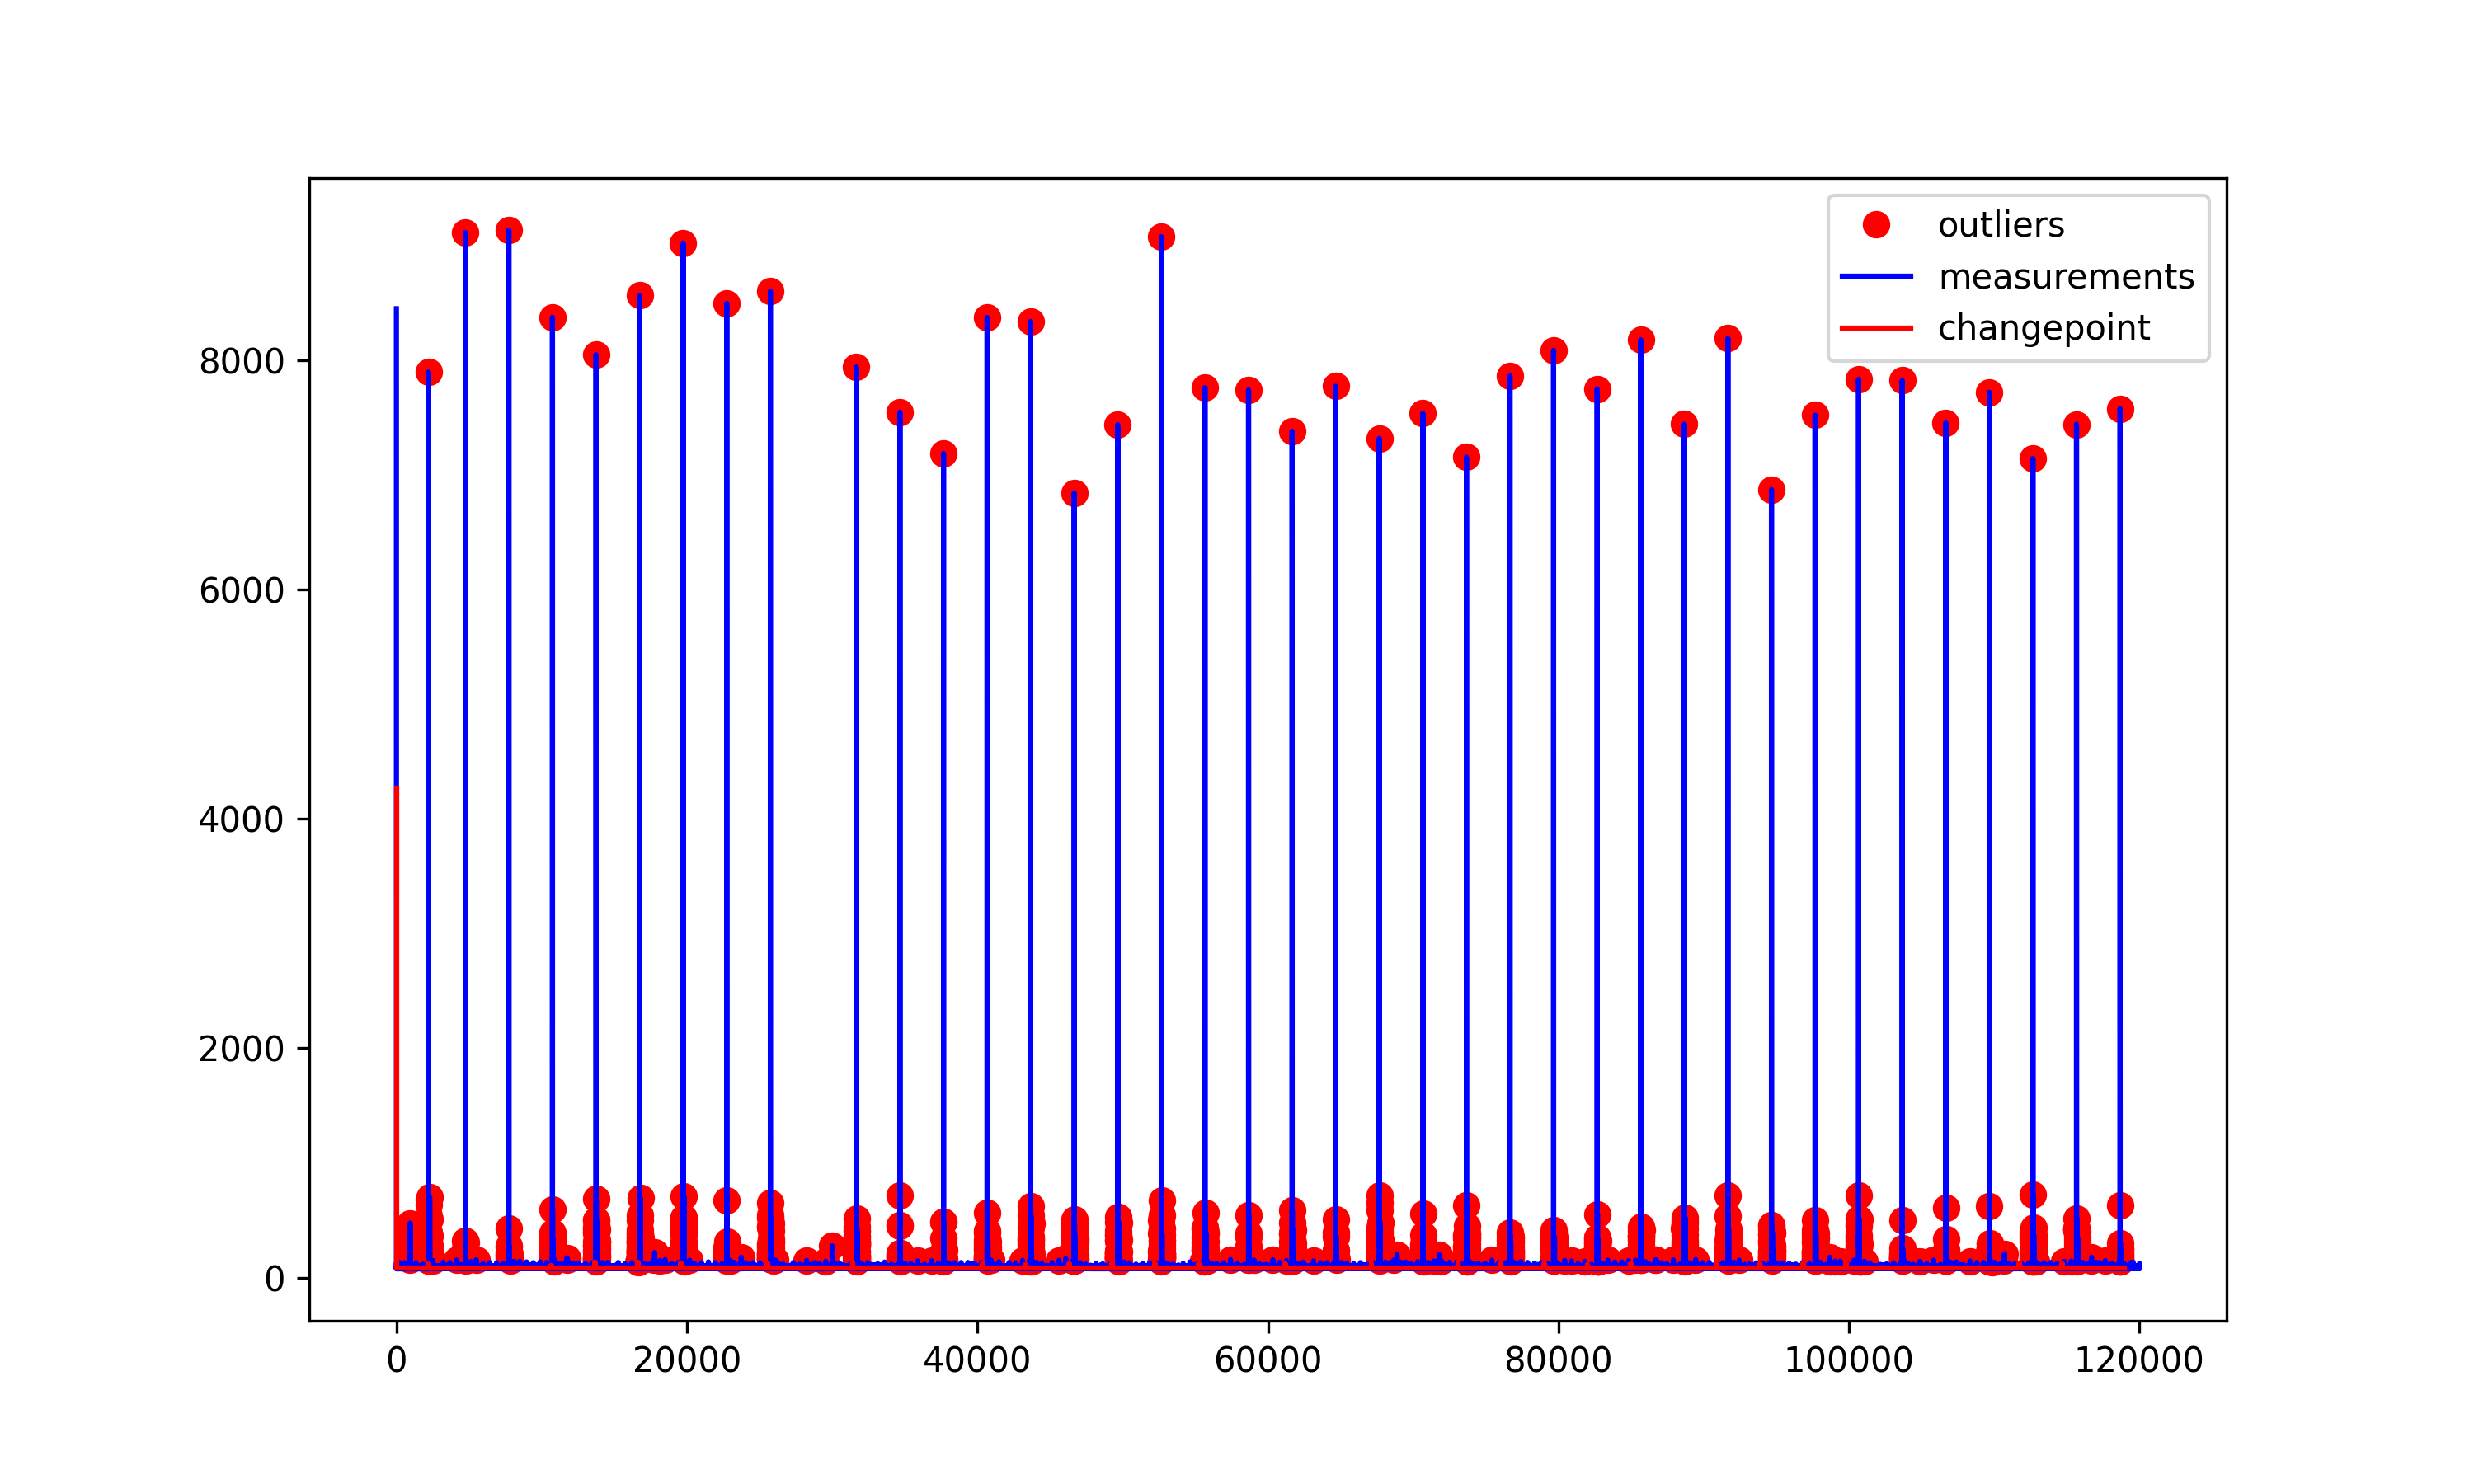
\includegraphics[width=1\textwidth]{images/plot_13_flat.png}
    \caption{CD benchmark from Node classify as warmup affected mostly in means}
    \label{fig:bench_node_flat}
\end{figure}

For example the problem here from the previous techniques with rolling window is that it does'nt remove the first outliers because it ignore the 200 first measurements but you could have some outliers in this part of the measurements. So I'm trying to find a better techniques to remove those outliers.

Anomaly detection consists in highlighting data with a different behavior from the majority of the data. 
Indeed, the detection can be performed in supervised mode in case information on the normality of the data is available which is not the case here because it would means to labelising the outlier inside the rebench Data. In other words, any data in the learning base can be labeled as normal or abnormal. In semi-supervised mode, the training database is assumed to contain only normal data. 
As for the detection in unsupervised mode, no information on the normality of the data is available which the case here and the case in the \cite{barrett2017virtual} Paper. 

\subsubsection{Unsupervised techniques}
The unsupervised approach is the most suitable for anomaly detection problems and benchmarks data. In this approach, the different algorithms try to distinguish aberrant observations by learning about the data set, without having the labels of the observations: there is no set of observations identified a priori as anomalies. It is therefore not necessary to have labelled data and this simplifies the problem of preparing the data before learning and all the difficulty in constructing labels. In this section, I will briefly present some unsupervised techniques and their application with Rebench Data.

In the paper they apply the rolling window by removing all elements that are outside the mean by 15\% and 85\% They ignore the 200 measurements because it would remove too much interesting data about warmup which represent 10\% of the size of the whole benchmark in their paper. There was some problem with outlier removing because in the rebench data there was clearly outlier that past the warmup phase should be removed, so I reduced the ignore phase to 5\% (100 first measurements for a benchmark of 2000 measurements  which are ignored).

\subsection{Classification}


There was some problem with the classification I adapted the algorithm which works now depending on the size of the benchmarks.
The classify function from \cite{barrett2017virtual} takes as parameters the measurements from rebench and the length of the measurements it is useful because otherwise, the STEADY\_STATE\_LEN would stay to 500 which is not suitable when the length of the measures are under 500 for example. After all, it would mean that the steady-state length would be more than the size of measurements which is not possible.

This code bellow is majorly from the \cite{barrett2017virtual} but is adapted in Python and vary the classification dynamically depending on the size of the whole benchmarks.
\begin{python}[h!]

# From paper Virtual Machine Warmup Blows Hot and Cold

import numpy as np


DELTA = 1  # Absolute time delta (in seconds) below which segments are
# considered equivalent.
STEADY_STATE_LEN = 500  # How many in-process iterations from the end of the time-series
# data will a non-equivalent segment trigger "no steady state"?


def percentage(percent, whole):
    return int((percent * whole) / 100.0)


def classify(segs, n_values):
    assert(len(segs) > 0)
    last_seg = segs[-1]
    STEADY_STATE_LEN = percentage(25, n_values) # Steady state when the data need to stabilize
    lower_bound = last_seg['mean'] - max(last_seg['variance'], DELTA)
    upper_bound = last_seg['mean'] + max(last_seg['variance'], DELTA)
    label = "flat"
    i = len(segs) - 2
    while i > - 1:
        seg = segs[i]
        i -= 1
        if seg['mean'] + seg['variance'] >= lower_bound and seg['mean'] - seg['variance'] <= upper_bound:
            continue
        elif seg['end'] > n_values - STEADY_STATE_LEN:
            label = "no steady state"
            break
        elif seg['mean'] < lower_bound:
            label = "slowdown"
            break
        assert(seg['mean'] > upper_bound)
        label = "warmup"
    return label
\end{python}





\section{Overview of Changepoint detection algorithm}


So first I used a package which allows me to do changepoint analysis which is called ruptures \cite{truong2020selective}, it works well, but after reading the warmup paper I prefer to use the algorithm from R "changepoint" \cite{killick2014changepoint} in order to reproduce the experiment.



\subsection{Changepoint Detection}
In statistical analysis, the changepoint detection problem is a regression problem to estimate the times at which a signal exhibits changes in the distribution. . Classically, changepoint detection is performed for a signal with changes in the mean. More generally, changepoint detection is performed for a signal with changes in the distribution (for example, in the mean and variance). \\

Changepoint  detection can be applied to a sound signal of a program for which we wish to estimate the moments when situations change, to the detection of computer attacks  , or to quality control, here for the rebench Data it help to classify behaviour in warmup analysis. \\

This next will deals with the problem of detecting changepoint retrospectively (known as offline) when all the signal data are available. This context is different from a real time detection (online) where the signal data arrive on the fly it could be interessting to classify on the fly after reaching  and classifying a stabilisation of a benchmark and stoping recording the benchmark data in order to save time , but online detection is less able to detect precisely the moment of rupture.

\subsection{Offline detection Parametric and Non Parametric}
 
 
Theire two big families of offline detection algorithm

\subsubsection{Parametric}

Advantages: speed of calculation, ease of interpretation and prediction,
good speed of convergence, possibility of validation;
Disadvantages: a priori choice of known functions (example: degree of polynomial), adapted to a limited class of tendencies.

\subsubsection{Non-parametric}


Advantages: adaptability, not a priori on the type of trend;
Disadvantages: limits in interpretation, validation and prediction,
choice of window / smoothing parameters.



Of course, there are very different ways of proceeding to analyze this type of signal. One of the most "intuitive" is to cut the series into "homogeneous" segments. This notion of homogeneity can cover, for example, homogeneity in mean, or homogeneity in variance (or homogeneity in mean-variance!).

There is 3 type of detection of Changepoint

Changepoint in mean, Changepoint in variance, and Changepoint mean or variance

In the paper \cite{barrett2017virtual} They used mean and variance detection with the changepoint algorithme



\begin{figure}[h!]
    \centering
    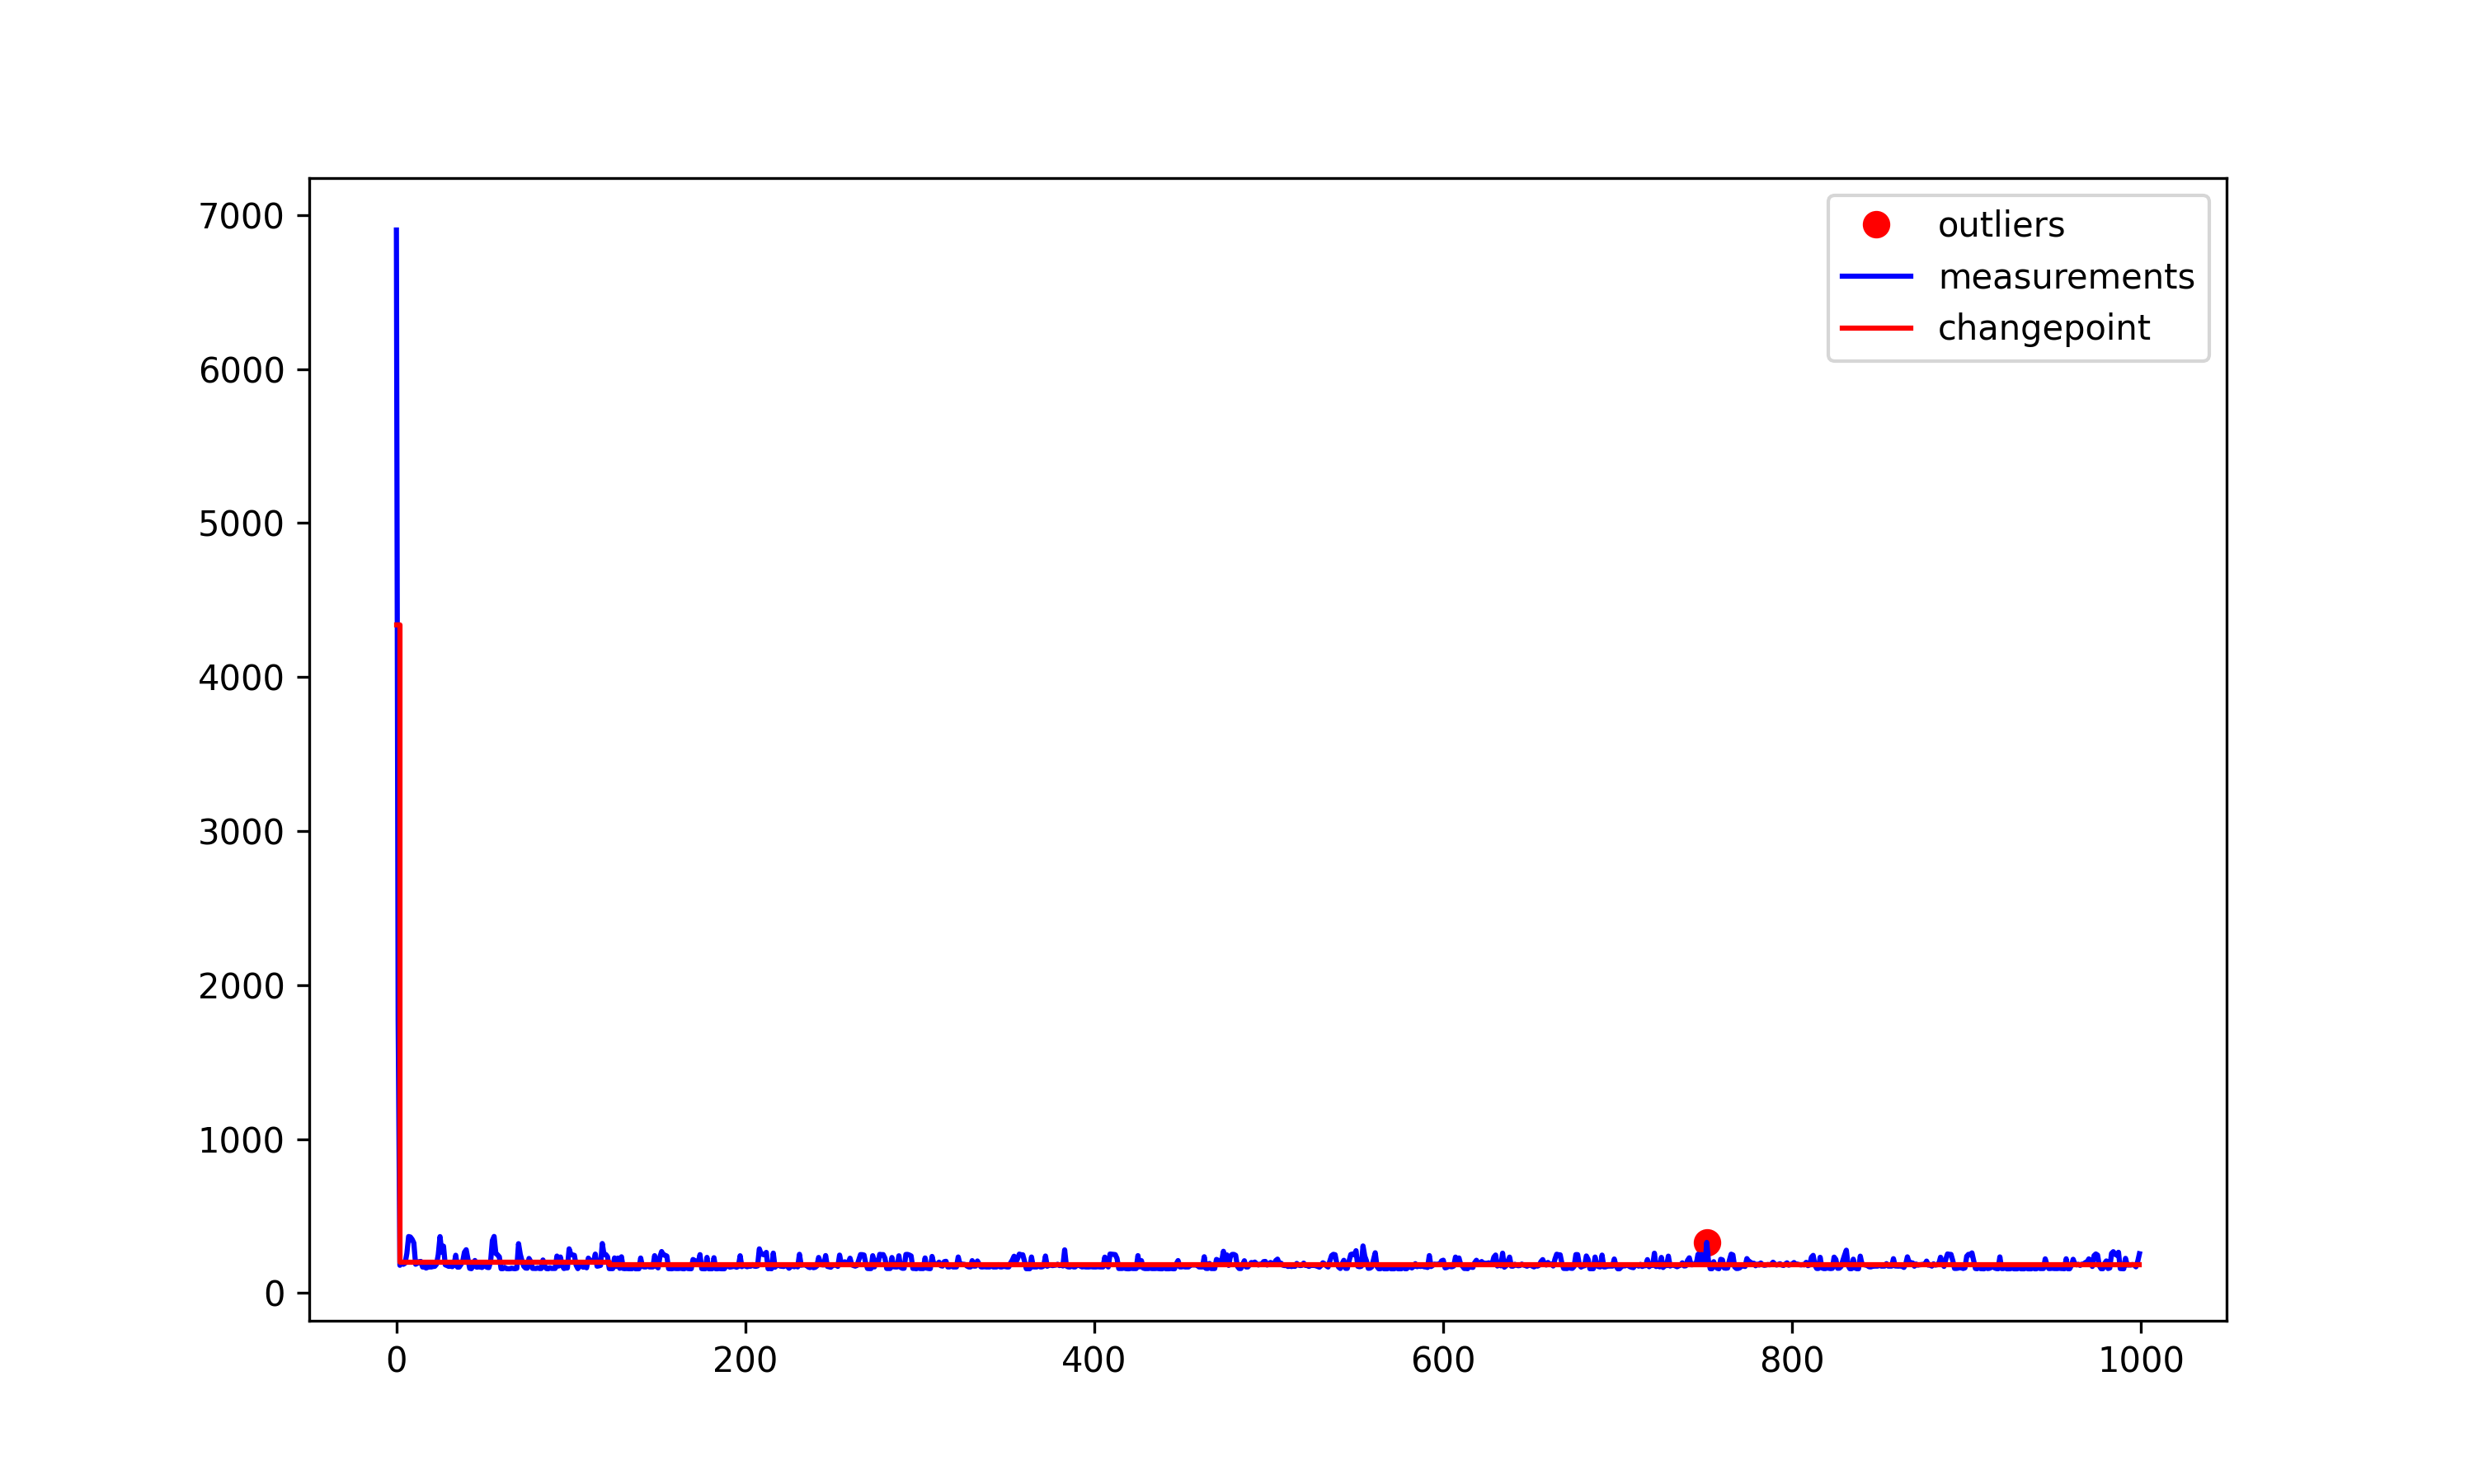
\includegraphics[width=1\textwidth]{images/plot_6_flat.png}
    \caption{CD benchmark from Node classify as warmup affected mostly in means}
    \label{fig:bench_node_flat}
\end{figure}



\begin{figure}[h!]
    \centering
    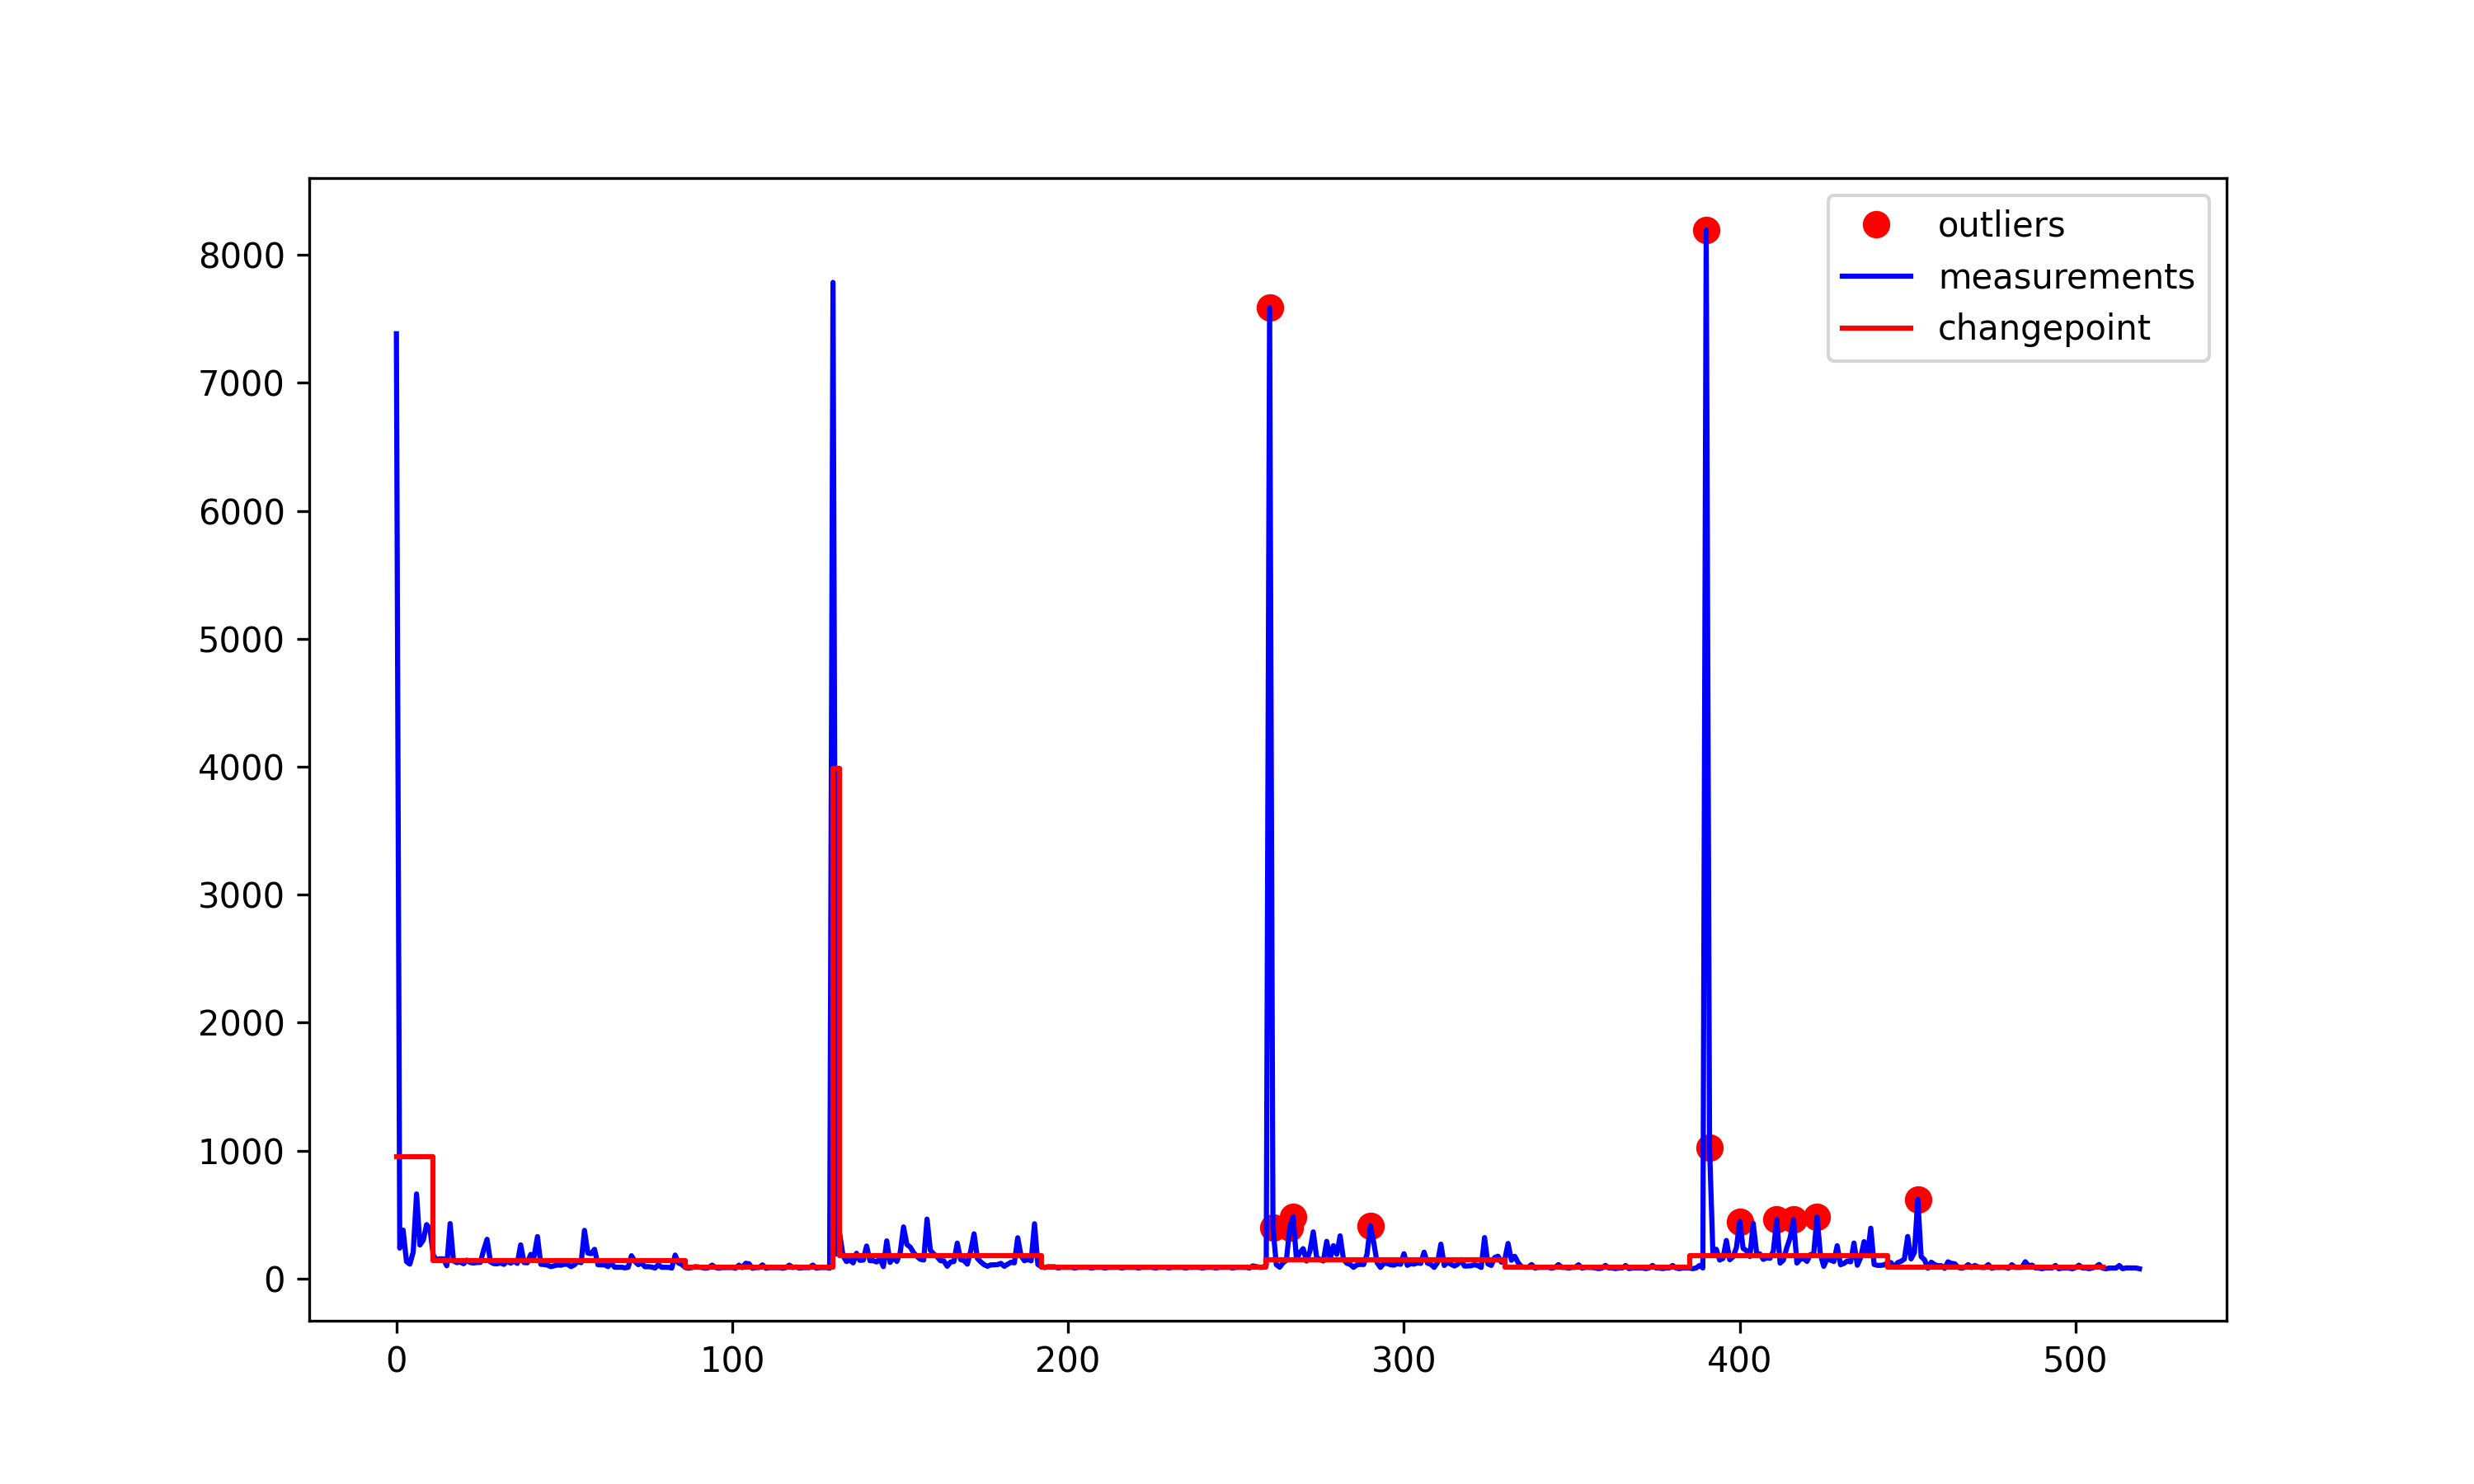
\includegraphics[width=1\textwidth]{images/plot_10_flat.png}
    \caption{CD benchmark from SOMns classify as warmup affected mostly in means and variance}
    \label{fig:bench_somns_flat}
\end{figure}

For example, for the two benchmarks above, it looks like:

the \ref{fig:bench_node_flat} series is affected by changes in the average,
the \ref{fig:bench_somns_flat} series by changes in mean and variance.


Based on these models, here is the kind of segmentation that could be proposed:

The above results are actually obtained using the changepoint package from \cite{killick2014changepoint}.

In the warmup paper they discuted three different functions:

cpt.mean which is used to detect changepoint in the mean (assuming that the variance is constant)
cpt.var which is used to detect  in the variance (assuming that the mean is constant)
cpt.meanvar which is used to detect changepoint in both the mean and the variance
These three functions are largely configurable. One can thus vary (among others)

The nature of the algorithm used to detect "optimal" breakpoints...
the type of test used to locate the changepoint (one can either assume that the residual distribution of the variables is Gaussian, or one can not make an assumption of distribution and use a non-parametric test)
the type and extent of the penalty applied in order to limit over-segmentation.

These aspects are discussed in \cite{killick2014changepoint}.

\subsection{Effect of parameterization}

Unsurprisingly, the above functions give very different results depending on how you set them up.

To choose the segmentation algorithm and other associated parameters, we will rely on 3 criteria:

Theoretical criteria (which model is best suited to the data? one with constant variance, one where the residuals are Gaussian, one that would account for segments of highly variable lengths, etc.).

Empirical criteria (I choose the method that gives the most "usable" results on real data, and the most correct results on simulated data). This is what i used because i assume that the data from \cite{barrett2017virtual} was verified and are correct.

Calculation criteria (the method must be computationally applicable for data of a certain size).

Obviously, determining which method is best using multiple criteria of these three types is difficult. Nevertheless, it is possible to discuss it by carrying out  the same type of study as \cite{leviandier2012comparison}. This could be a future work to find the best parameters for changepoint analysis for rebench Data but for this experiment I will stick to the parameters they used 





\section{ How to detect the change between benchmarks ? Overview of method to quantify difference between curve}

During this project I have review and try some techniques to quantify the difference between benchmarks and report if changement of behaviour as occure. During this dissertation i prefer to pick one benchmark problem which is the sleeping barber algorithm which is a sharing ressources problem in multi tasking.

\subsection{Sleeping Barber problem}
The program will have to be decomposed into two types of threads. On one side there will be the barber, represented by a single thread looping continuously to see if a customer is waiting, take care of him if necessary or go to bed. On the other side there will be one thread per client, which will simulate the "physical" client. He will try to enter the shop, sit down if he can, get a shave, and disappear.
While our program will have only one barber, there may be as many customers as there are men on the planet (or at least as much space in memory). The client threads will therefore pile up, waiting for space to become available in the waiting room, and then the barber will take care of them.

\subsubsection{ What does the barber do?}
The thread symbolizing the barber will therefore be unique. It will be started when the program is launched, before any customer, and will loop back on itself for all eternity.
Here's what our barber will spend his life doing:

\begin{itemize}
    \item Is there anyone in the waiting room? If there is, I'll take care of him, if not, I'll go to bed;
    \item When a customer is there I take him to the chair;
    \item I shave him;
    \item I give him the day off.
    \item Of course, when we get to the end, we loop back in.
\end{itemize}

\subsubsection{ What does the customer do?}

Here are the actions that the thread symbolizing each customer will perform. If there are several customers, identical threads will compete with each other:

\begin{itemize}
    \item I look in the hairdressing salon to see if there's any free space. If there is, I go inside, if not, I wait;
    \item When I'm inside I sit on a chair (and take my comic);
    \item I wait until the barber is free;
    \item I get up from my chair (and free a seat) and go into the room;
    \item I let myself trim my beard;
    \item When he's done, I pay and go home.
\end{itemize}

Looking at the difference in number of tasks between the barber's and the client's list of actions, we notice that the client does more things. In fact, the client has to manage an additional resource compared to the barber: the free place in the waiting room when he comes to the entrance of the salon.

\subsection{ Sleeping Barber experiment}

For running the comparaison between two curve I choosed four iterations of the experiment's of the sleeping barber problem implemention. The first one is a record one thousand iteration of the benchmarks and the second and the third one are a record of 5500 iterations their are from the project SOMNS, which is an implementation of the Newspeak Specification derived from the Simple Object Machine,

\begin{figure}[h!]
    \centering
    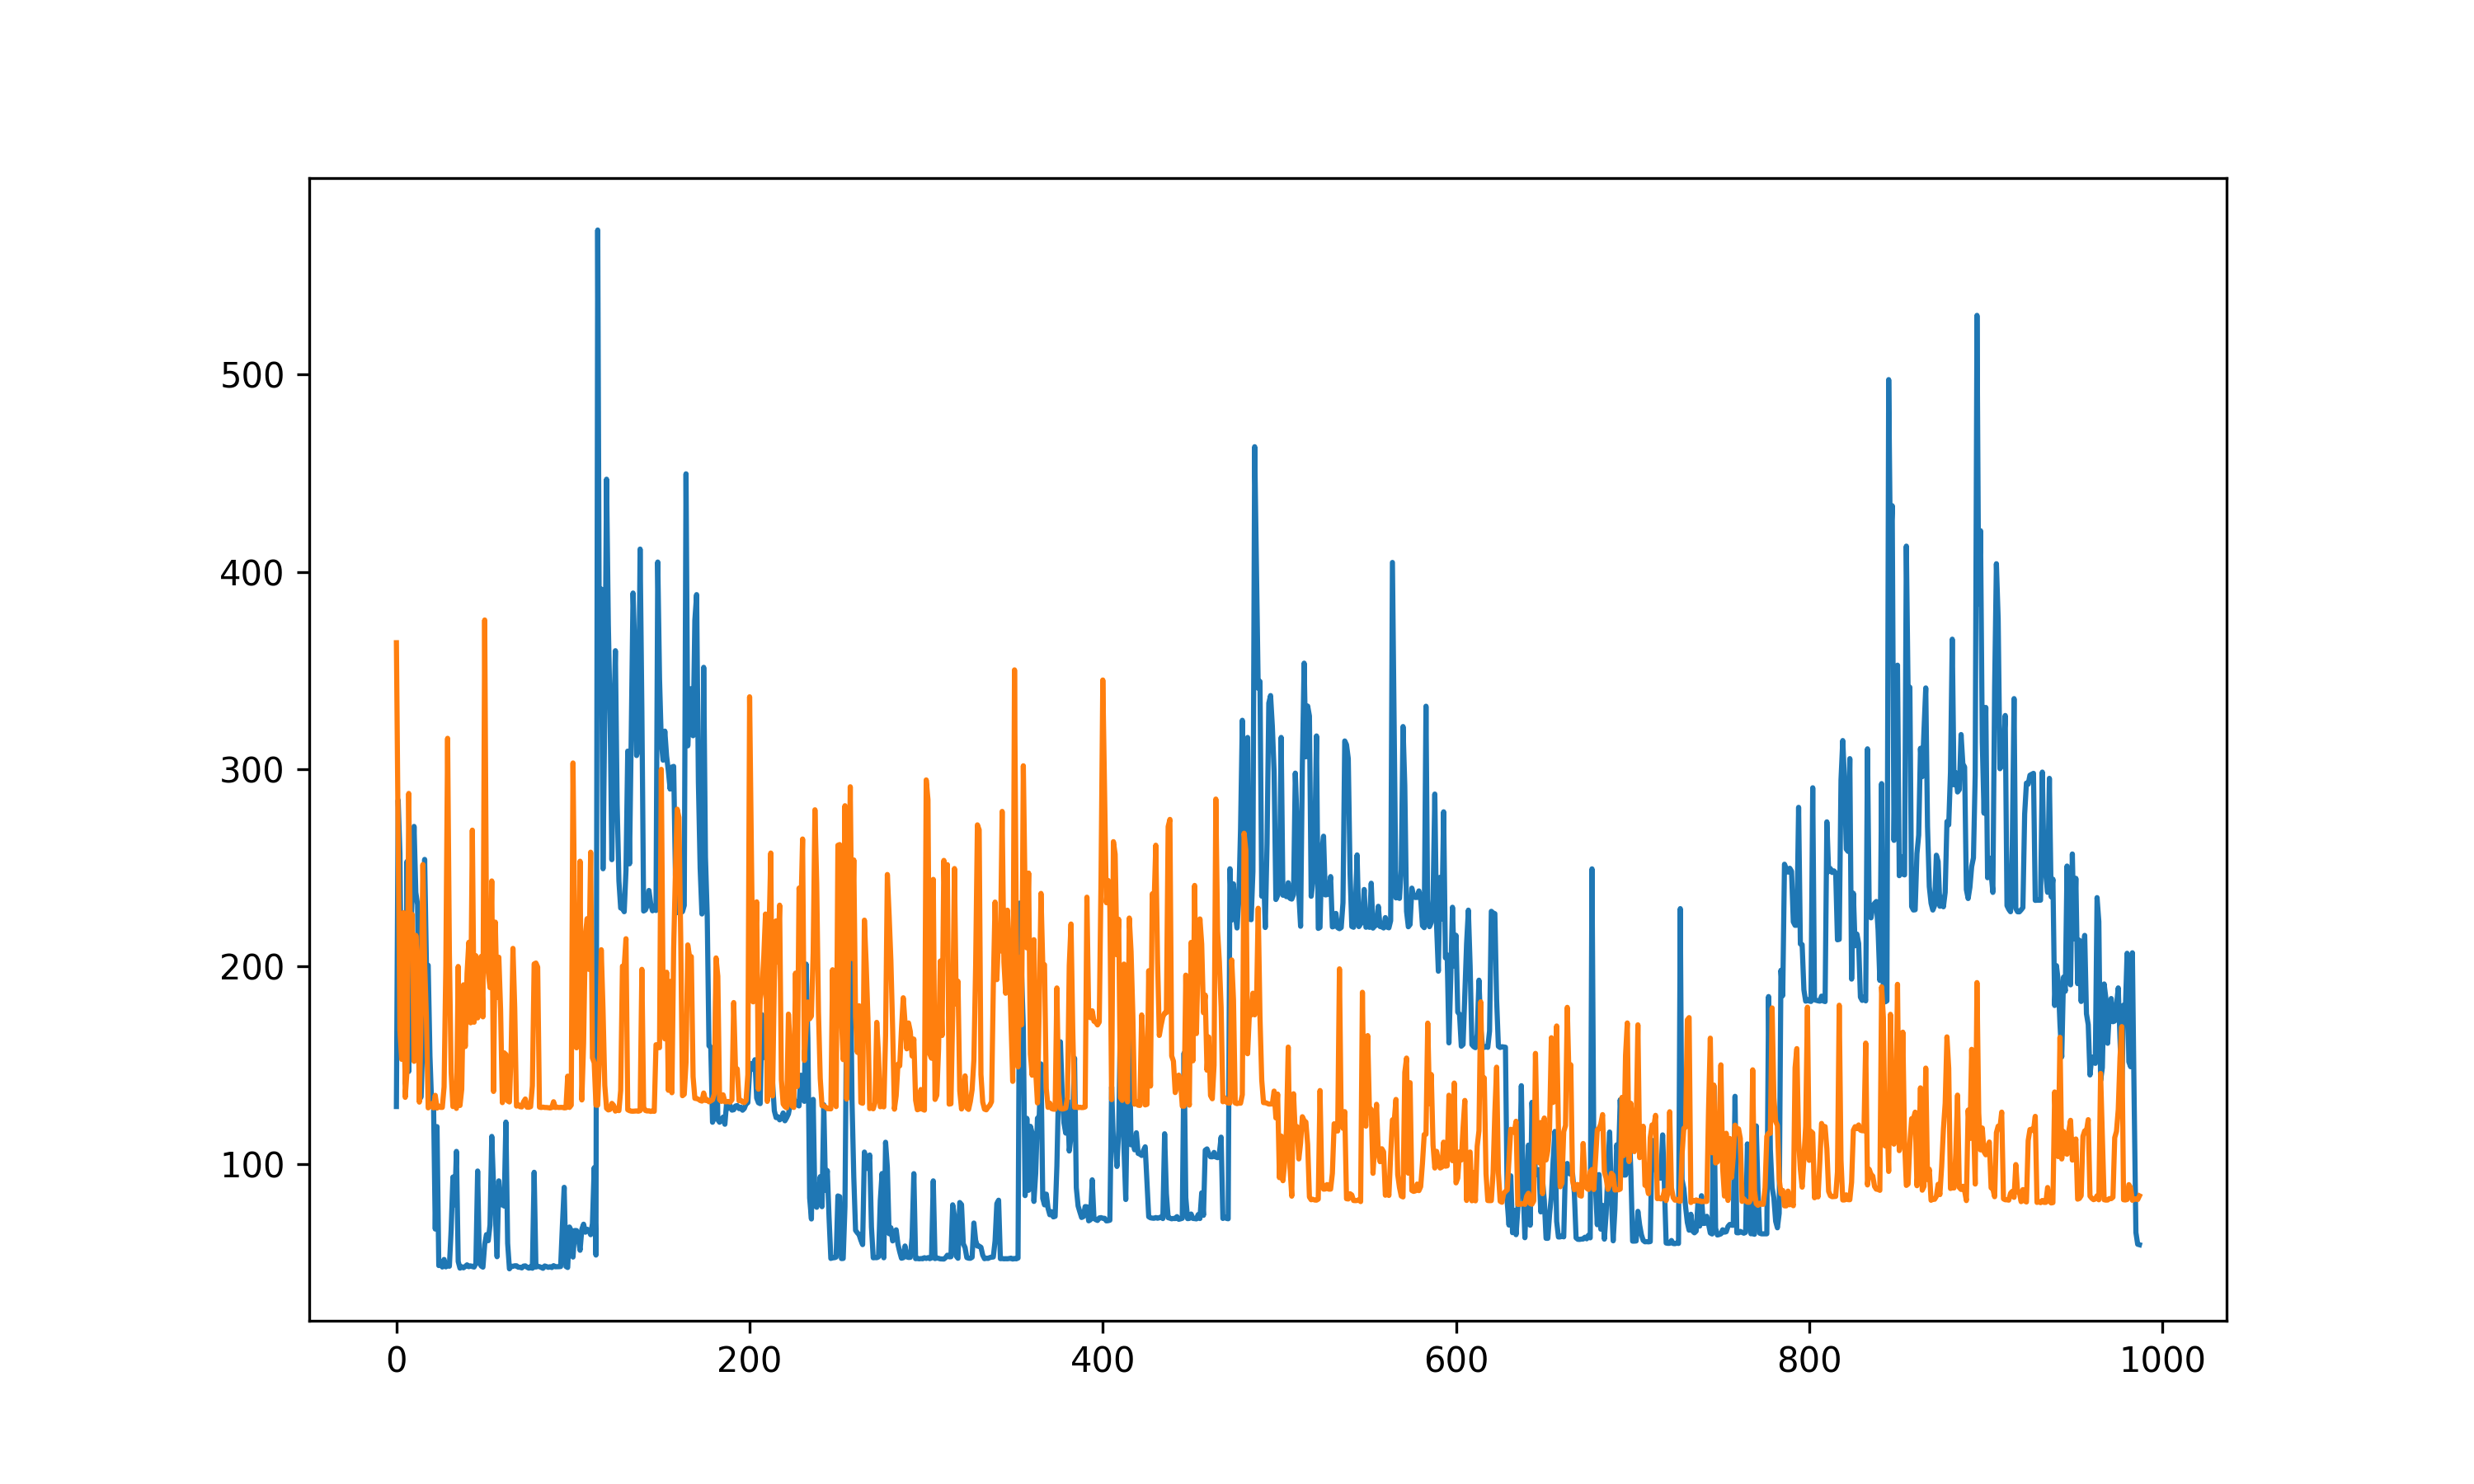
\includegraphics[width=1\textwidth]{plot_0.png}
    \caption{Benchmark 1 and 2 From sleeping Barber}
    \label{fig:bench_1_2}
\end{figure}


\begin{figure}[h!]
    \centering
    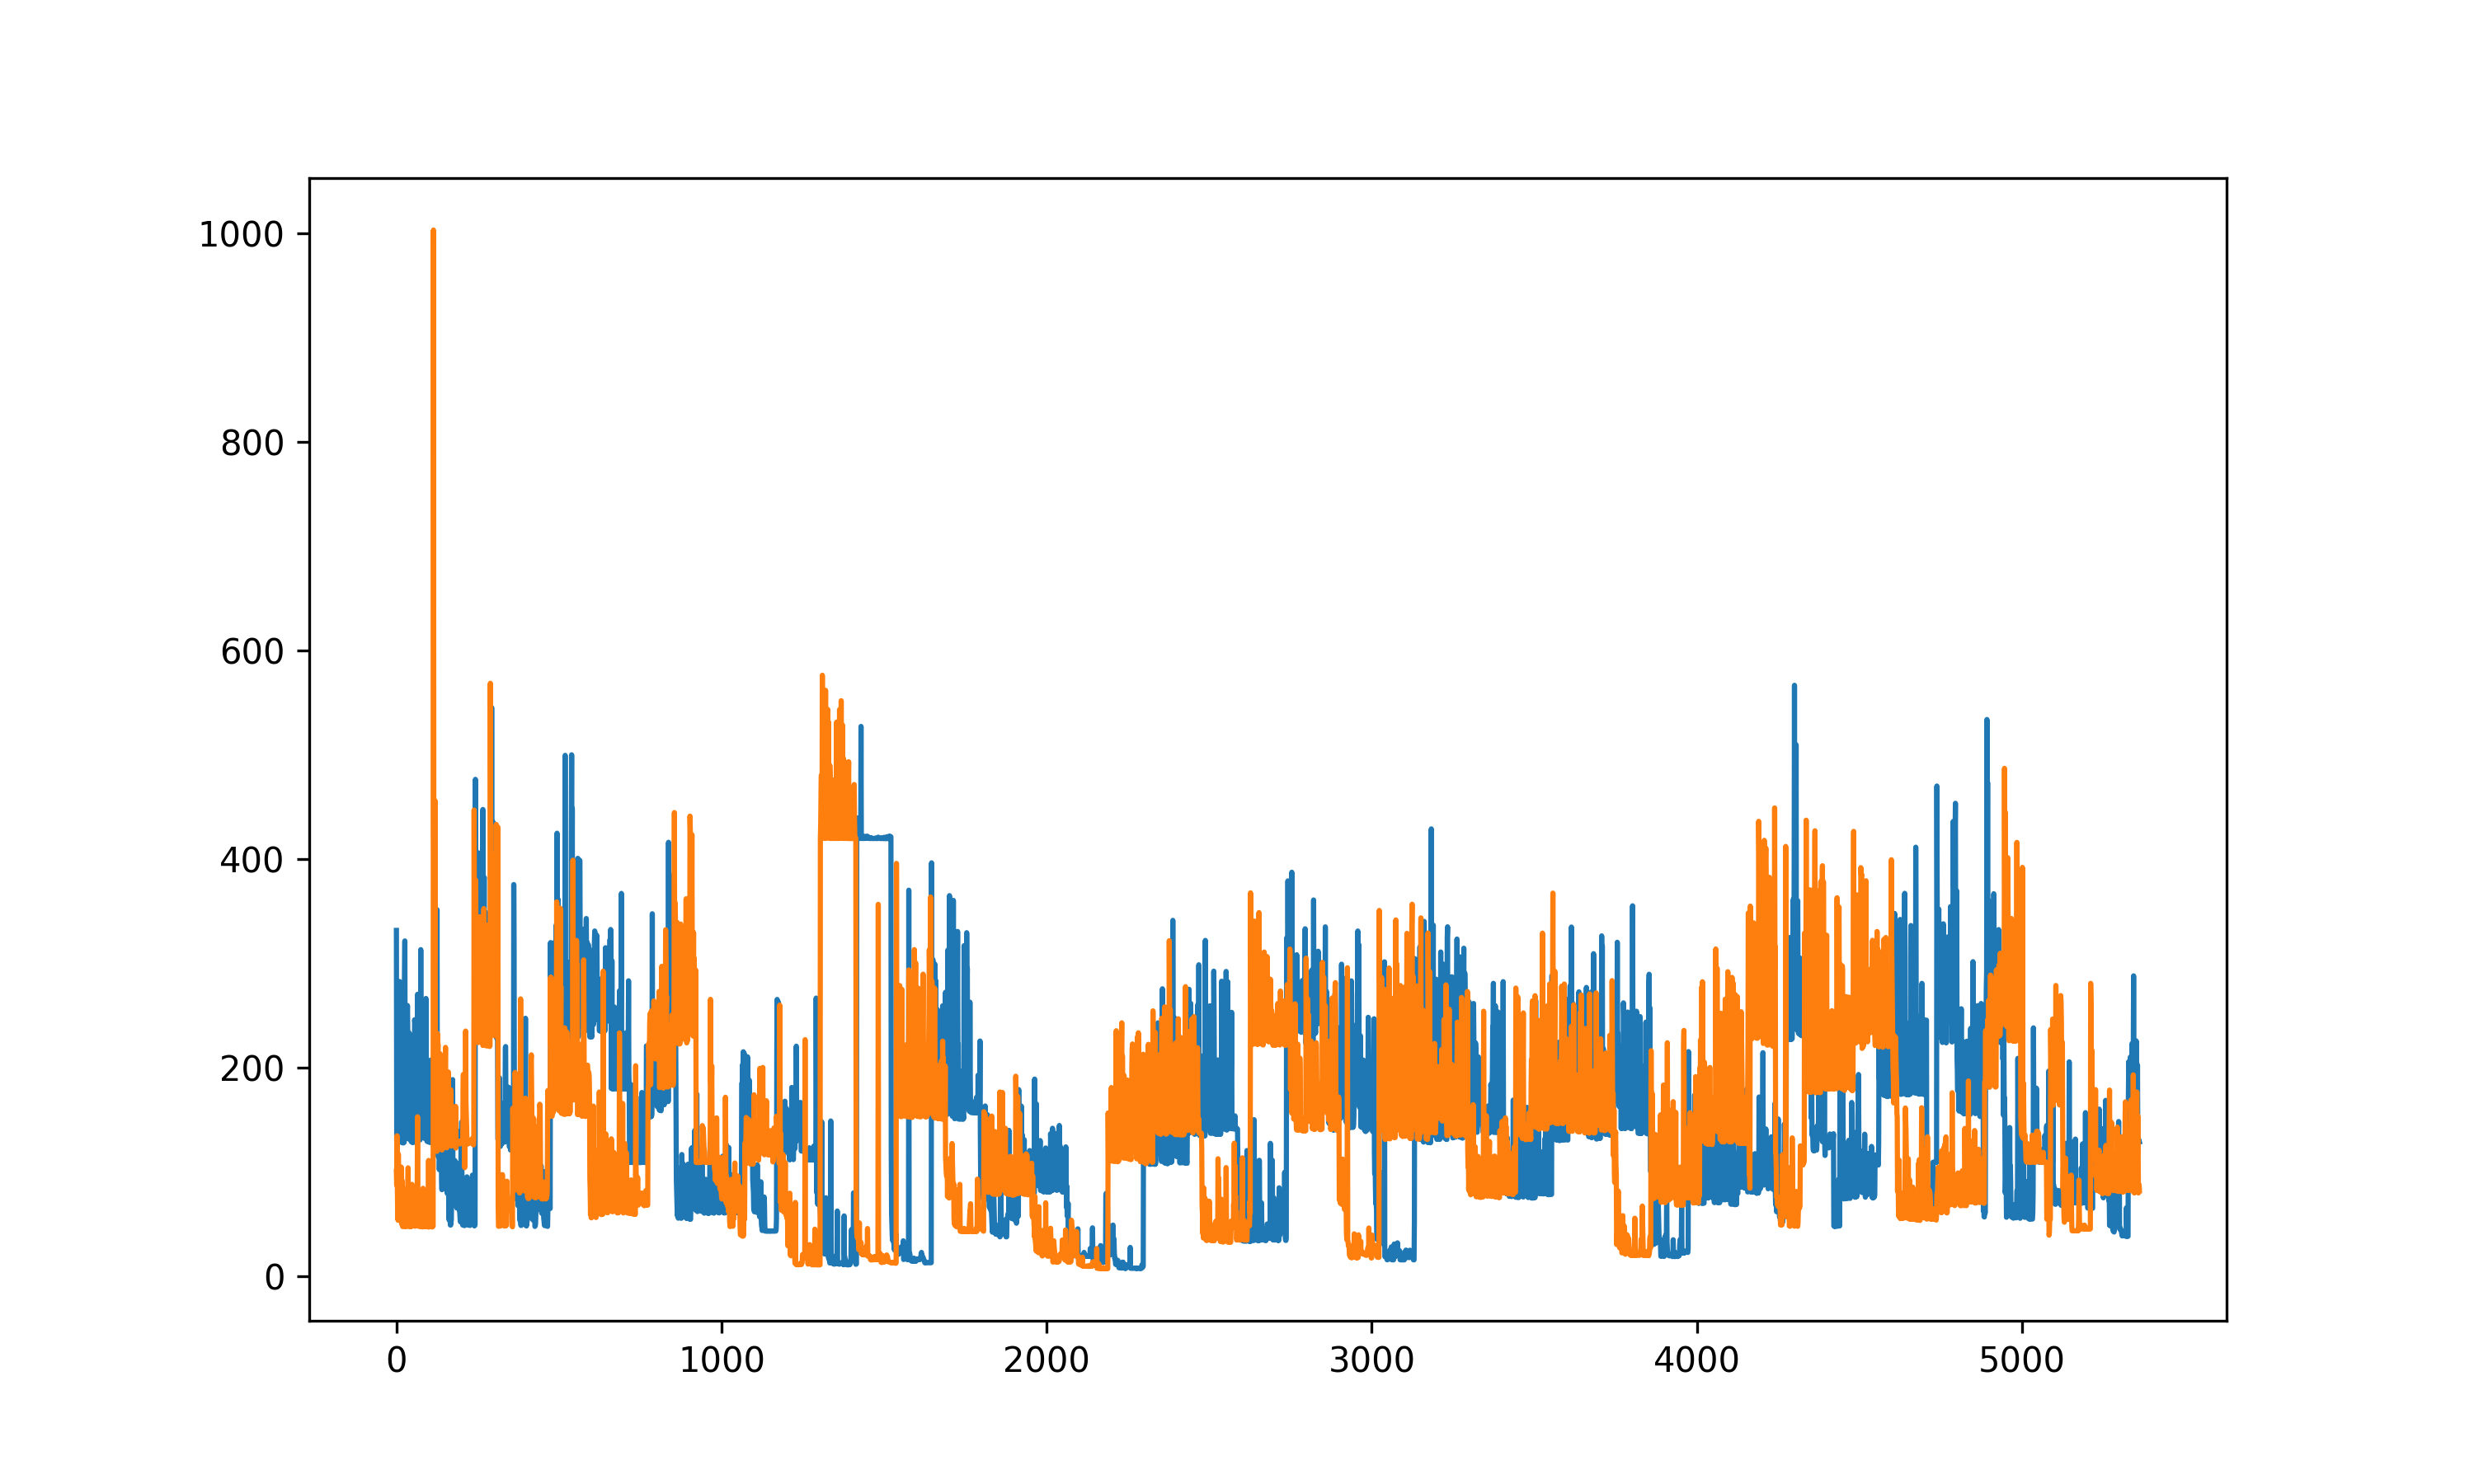
\includegraphics[width=1\textwidth]{plot_1.png}
    \caption{Benchmark 3 and 4 From sleeping Barber}
    \label{fig:bench_2_3}
\end{figure}

\subsection{Trying few curve comparaison algorithm}

The notion of distance is useful for quantifying and describing the objects present in
a curve for example. The desire to remain in the space of the image requires the use of specific distances, which provide exclusively integer results. After the definition of use, there is an inventory and a comparison of the main discrete distances used in curve analysis.

\subsubsection{Area method}

First i have used area \cite{jekel2019similarity} method to quantify the difference between curve, this an algorithm for calculating the Area between two curves in 2D space
Strictly speaking, the expression area under the curve refers to the area A of the domain delimited by a curve (represented in an x-y diagram) and three straight lines (the x-axis and two vertical lines with abscissa a and b). If the curve has the equation $y=f(x) y=f(x)$, the area is $A=\int _{a}^{b}f(x)\, {d} x$. This area is a true area (e.g. milliseconds for benchmarks) only if the function f has only positive (or zero) values over the interval [a,b] and if both the abscissa and the ordinate are lengths (with the same choice of unit, e.g. milliseconds for benchmarks).
For the purpose of detecting if the behaviour has change between two benchmarks its not interesting because it quantify the area a a whole and area can be equal but not their behaviour

\subsubsection{Curve Length Measure}

Let consider in the plane a curve which is the graph of a function f defined on the interval [a, b]. For example, the algorithm will calculate the length of this curve. To do this, we will approximate the curve by a broken line formed of n segments and calculate the length of this broken line. We will then obtain the exact length of the curve by a limit process.
Theoretically, the length of the curve representative of a
function f over an interval [a; b] (on which it is differentiable) is given by $\int_{a}^{b} \sqrt{1+f^{\prime}(x)^{2}} d x$
This makes it possible to obtain the exact value compared to the initial problem
as well as an approximate value and appreciate the accuracy of the algorithm
according to the value of n.

\subsubsection{Hausdorff Distance }
The Hausdorff distance is used to account for the maximum deviation between two polylines (L1, L2). By definition, two polylines L1 and L2 are at a Hausdorff distance (dH) from each other of less than d units, if each point of L1 is within d units of at least one point of L2, and if, reciprocally, each point of L2 is less than d units away from each other by at least one
point of L1.

The Hausdorff distance is defined as the greater of the two following components :

\begin{itemize}
    \item d1 which is the largest value of the non-symmetrical distance from L1 to L2,
    \item d2 which is the largest value of the non-symmetrical distance from L2 to L1.
\end{itemize}


This distance has the advantage of providing two measurements. Right-of-way lines can thus be compared using the component starting from the most short line. On the other hand, the Hausdorff distance, with the disadvantage of calculating the
distance on the nearest pairs of points and not on homologous points. Homologous points are points that visually correspond to each other. For example, the point in L2 used to calculate d1 is not the Intuitively corresponding to the point of L1, it is simply the closest point. The distance from Hausdorff considers polylines as simple sets of dots unordered. This problem is particularly important for very sinuous or with loops. Small distances can then be sent back to dissimilar lines. Similarly, pairs of dots cannot be considered to be matches. Nevertheless, this particularity has the advantage of
reduce calculation time: the algorithmic complexity of this algorithm is linear. 

This methods seems to be working better because there is no need for the dataset to know if the first clue of the first sequence must match the first clue of the other sequence and that
the last clue of the first sequence must match the last clue of the other sequence (but it must not be its only match).

\subsubsection{DTW}

 The DTW finds the best match between a reference (the score) and a signal (the interpretation) by calculating a difference between vectors of the characteristics for each of these signals. The comparison algorithms of chaines are based on the exact correspondence between the reference and the signal and do not take into account, among other things, the imprecision of the pitch estimation due to chords or errors of the height detection algorithm. In addition, the DTW can be used to align continuous multi-dimensional characteristics, for example results from a signal analysis, which allows the partition alignment to be based on parameters such as the number of partitions, the size of the partition, the number of partitions, the number of partitions to be aligned, the number of partitions to be aligned, the number of partitions to be aligned, the number of partitions to be aligned and the number of partitions to be aligned.
The system does not require prior segmentation of the benchmark measurements and does not require prior segmentation of the
signal.
In short, the DTW algorithm consists of three steps:

\begin{itemize}
    \item Calculation of local distances
    \item Dynamic programming to obtain the global optimum \begin{itemize}
        \item a) Calculation of increased distances. Only the minimum predecessors are kept. of each point => local optimum
        \item b) Backtrack to find the minimum distance => global optimum
    \end{itemize}
    \item Result: A shift path that consists of the correspondence of the two equations.

    
\end{itemize}

\subsection{Interpretation of results after running the algorithms}

After Choosing the two benchmarks I ran each algorithm on each experiments of the barber problem.
The 1 \& 2 experiments are not similar in contrary of the 3 \& 4 which are similar by human eyes.
Each output of each algorithm are put inside this tabular

The first result is about the fréchet distance which is the minimal length  between two point of the two curve which is sum  for every point of each experiment that we are comparing.

The second result is the area difference of the two curves (bigger number mean bigger area difference).

The third result is the total lenght difference of the two curves (bigger number mean bigger length difference).

The fourth result is the cost which is the sum of absolute differences, for each matched pair of indices, between their values.

The last result is the sum of each pair of the distance subsets are from each other.

\begin{table}[h!]
\begin{tabular}{|l|c|c|c|c|c|c|}
   \hline
   benchmarks  & area & curve length & DTW & directed Hausdorf \\
   \hline
   1 \&  2 & 313 & 81918 & 14 & 68757 & 197\\
   \hline
   3 \& 4  & 295 & 32960 & 48 & 191649 & 7 \\
   \hline
\end{tabular} \\ 
\caption{Comparaison between two inequal benchmarks and two equal benchmarks}
\end{table}


As expected the only algorithm that seems to work is the directed Hausdorf algorithm because it is not influence by the size of the dataset, indeed as the curve lenght increase the difference of the score increase. 
I order to classify if a benchmark has changed between 2 commits, I have to found a threshold where, if the result of an algorithm would surpass this threshold it will means that the benchmarks has changed from the previous commit. I order to get that threshold i labelised by hand all the benchmarks by hand. For 50 benchmarks by hand 6 have a real changed by human eyes and the rest have not changed between commit. Those 50 benchmarks could be corresponding to our training data. The threshold that seems to better classify is 20 because based on that the result of the directed hausdorf algorithm is that value that is better to separate the behaviour changed benchmarks and those who have not changed.
I have put a threshold of 20 with the directed Hausdorf. When the directed Hausdorf value is more than 20 is interesting to look at the benchmark because it means that their is significant difference between the two benchmarks.

\subsection{Conclusion of classification of variation of behaviour between benchmarks}

The validation of an unsupervised classification, as well as the choice of the number of group always remain open questions. On real data, recognized criteria such as the distance difference or the silhouette index are optimal with only two groups, limiting the contribution of such an analysis.
Future work might be to automaticly finding the threshold without labelising the data by hand and finding the best threshold for the quantify algorithm.
I could be interesting to apply the directed hausdorf to more use case than the sleeping barber experiment



\section{Setup Of Rebench Data}

\subsection{Building a rest API around the database Structure}

First thing I did was take the data collected  which is produced by rebench \cite{ReBench:2018}. The data is format in Postgres SQL format which is a language for communicating with a database. This computer language is notably very much used by web developers to communicate with the data of a web site (Here an REST API).

To import the backup of the data produced by Rebench I am using this command which will import only the data and not the structure which it created by the node.js server.

\begin{python}[h!]
pg_dump --verbose -Fc -U postgres -h 0.0.0.0 -p 5432  -a --dbname=postgres > data.dump
\end{python}

THe structure was designed by \cite{ReBench:2018} but i am including a map of the structure to see it more clearly.


\begin{figure}[h!]
    \centering
    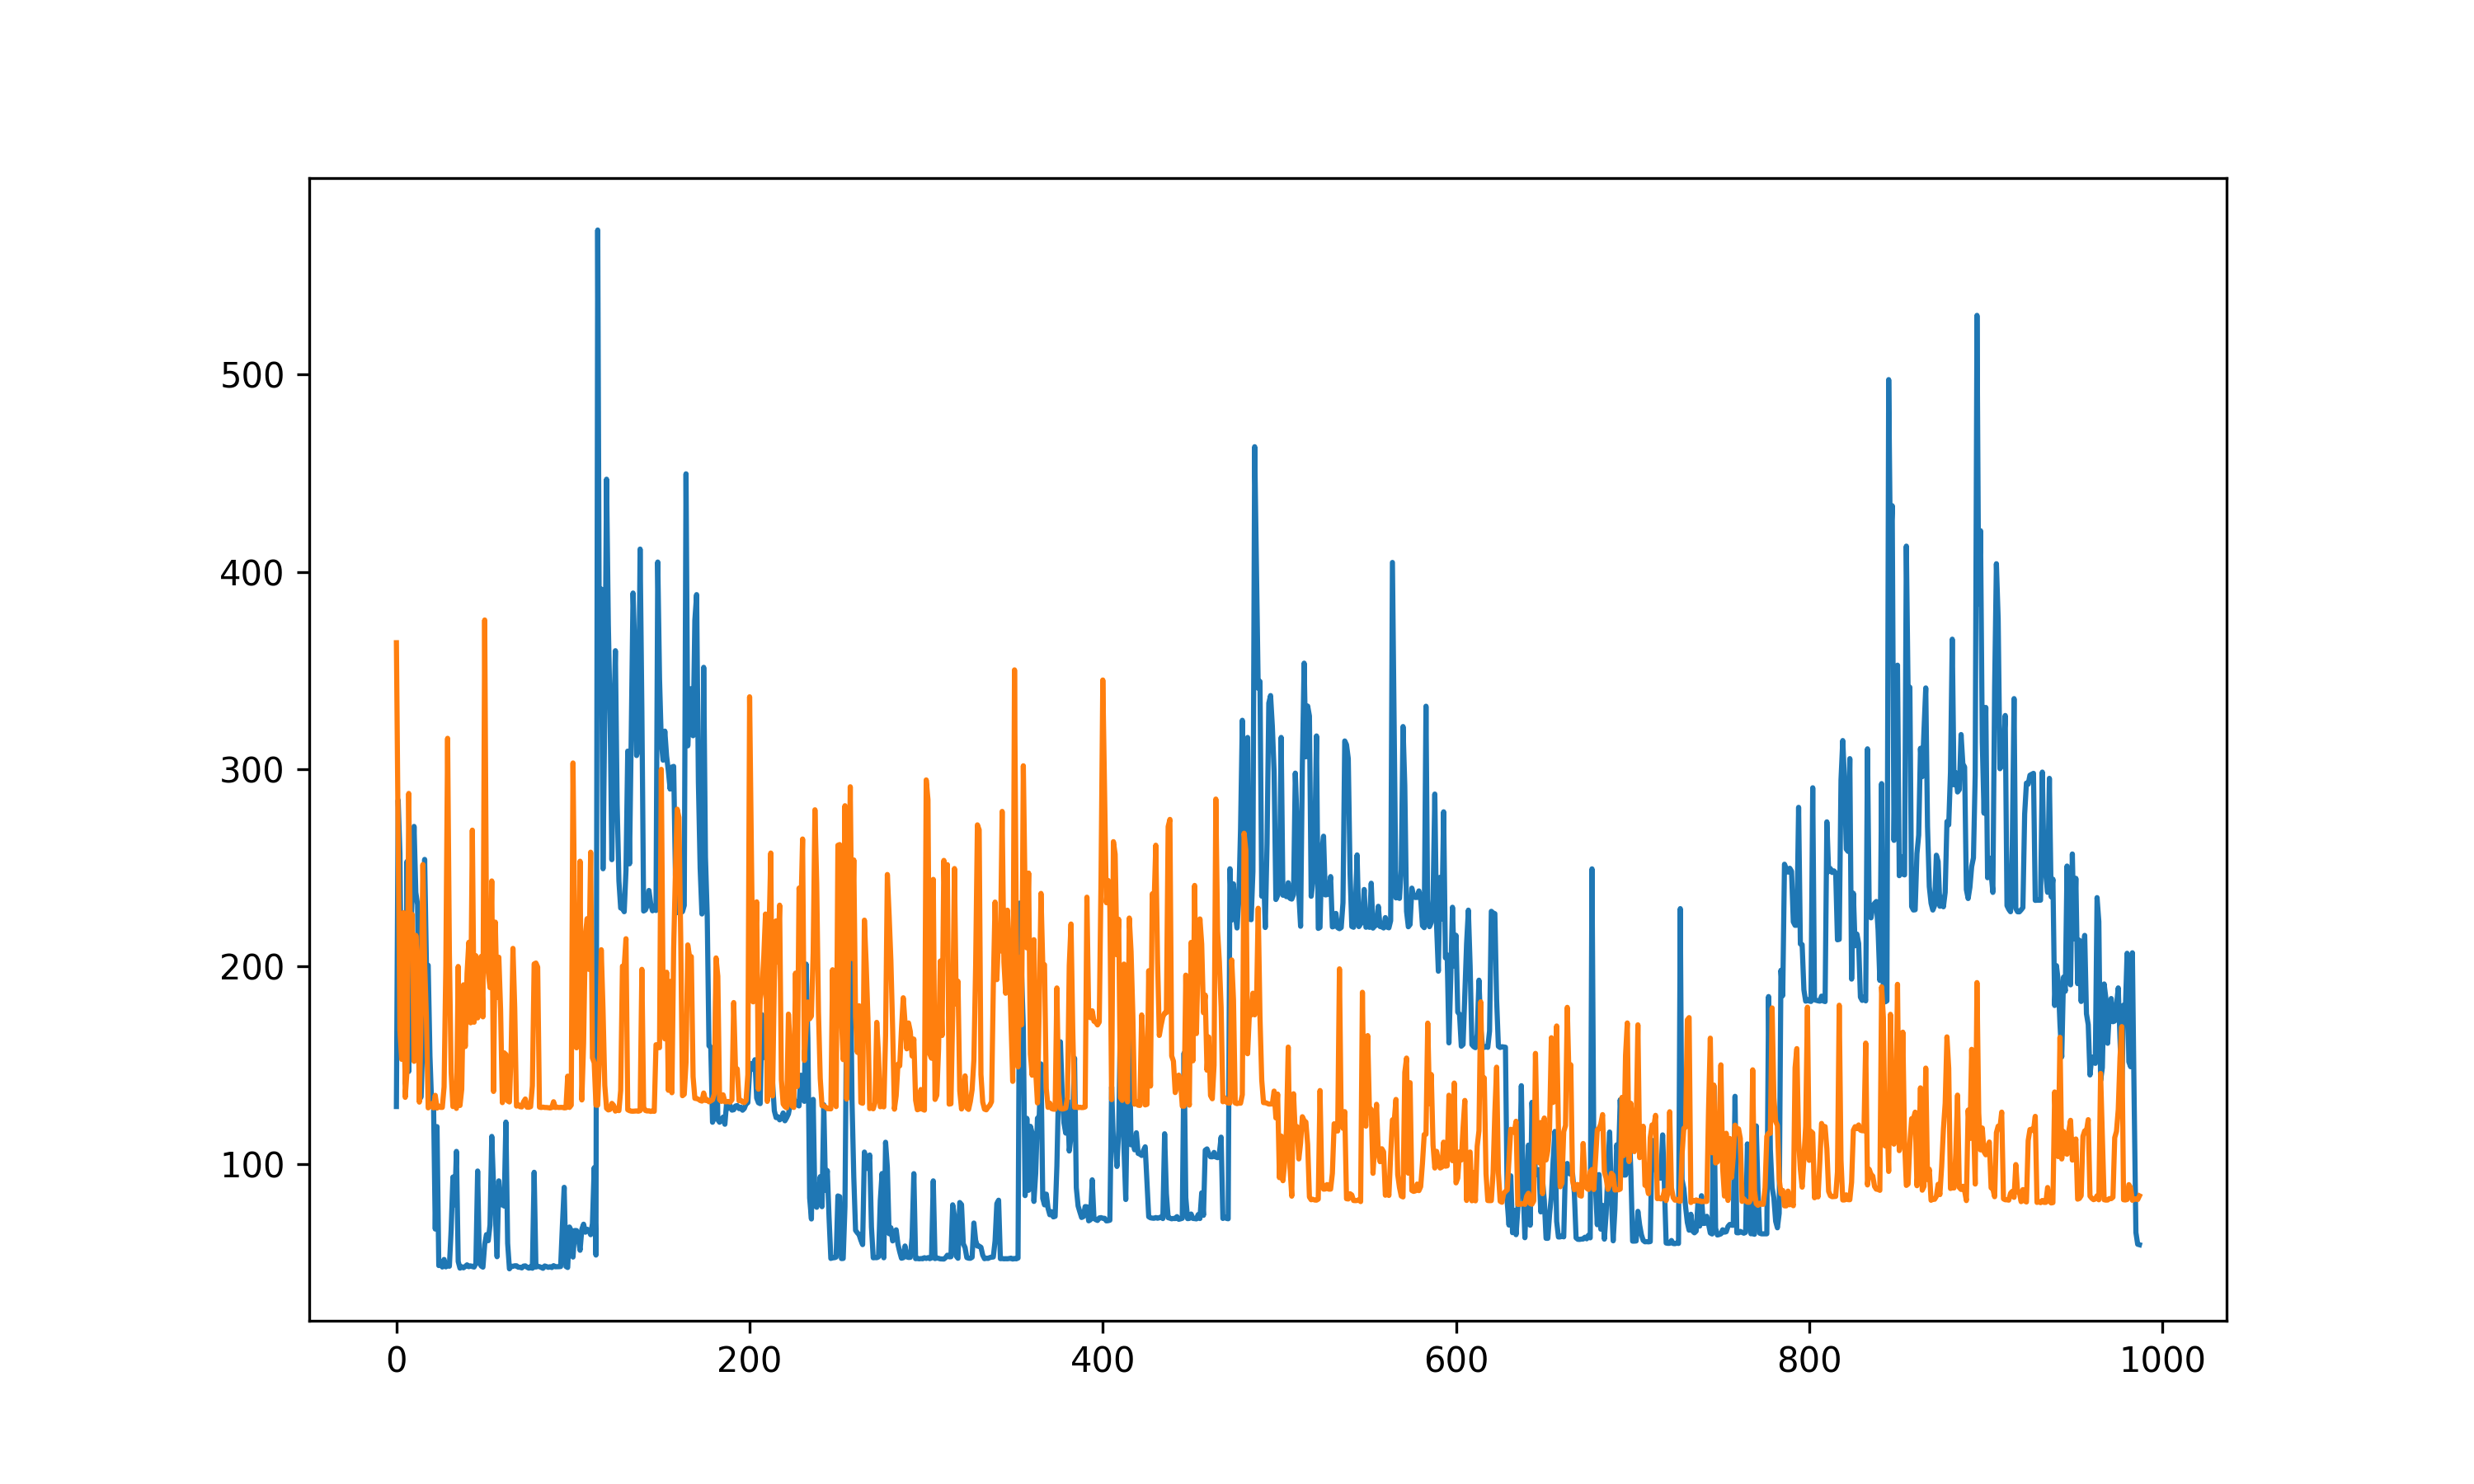
\includegraphics[width=1\textwidth]{plot_0.png}
    \caption{Benchmark 1 and 2 From sleeping Barber}
    \label{fig:bench_1_2}
\end{figure}




The database is runned in a docker container I will explain it later.

After that I needed to manipulate the so I build a REST API which is  a style of architecture for building applications. It is a set of conventions and best practices to be respected and not a technology in its own right. The RESTful architecture uses the original HTTP protocol specifications, rather than reinventing an overlay .

\begin{itemize}
    \item The URI as a resource identifier
    \item Using HTTP verbs as operation identifiers (GET, POST, PUT...)
    \item HTTP responses as resource representation
    \item Links as a relationship between resources
\end{itemize}

To communicate with the database I'm using an ORM (Sequelize) between the database language SQL and the javascript side \cite{pereira2016working}. ORM or Object Relation Mapping is a mapping process between objects and relational database systems. An ORM (here Sequelize) acts as an interface between two systems (Postgresql and The node.js Server). ORMs offer to the developers basic benefits, such as reducing time and effort and focusing on business logic. The code is robust instead of redundant. ORM helps manage queries across multiple tables efficiently. Finally, an ORM (such as sequelize) is able to connect to different databases (which is useful when switching from one database to another).

\subsection{}


\subsection{Deployement with Docker}

To deploy the application, I use Docker; this is an open-source software platform to create, deploy and manage containers a container image is. It is a set of light and independent software processes, gathering all the files necessary for the execution of the processes: code, runtime, system tools, library and parameters. They can be used to run Linux or Windows applications. So I dockerised the app to make it easier to deploy in the future. I also use docker-compose, it's a tool that allows to describe (in a YAML file) and manage (in the command line) several containers as a set of inter-connected services. In this application, I describe a set composed of 3 containers: Postgresql, the server node.js for the REST API and a python notebook to present the data. In the beginning, Docker was only used to manage the local working environment, for example, dependencies like PostgreSQL, which allowed me to separate the data from other databases on my computer.

The stack of the project in production is launched like this in production; it builds and launches Docker and does the network mapping between them.

docker-composes -f docker-composes.yml -f docker-composes.production.yml up --build -d

You can see the docker-compose-.yml file in the Github repository \url{https://github.com/Vatoth/master-thesis}. 

Because of the data is created by rebench is from a postgresql database the goal is to add a postgresql connection so that we can retrieve information from a database and display that information in the application as a simple list.
We will use MySQL as the database. For this, we will use an ORM (Object Relational Mapping). There are several ORM nodejs such as: sequelize, typeORM and mongoose. The most suitable ORM in our case is sequelize. Sequelize allows the use of a database type: MySQL, Postgres, SQLite and Microsoft SQL Server but for this project we will stick to Postgresql.

\section{Future Work}

How can you use the work from this disseration.
The first things that might be good to look at, is to integrate the report to github. There is a new  at github which is  actions \url{https://docs.github.com/en/actions/language-and-framework-guides/using-python-with-github-actions}
After triggering the CI by commiting to the project would be after the ReBenCh run take the data by the commit from the RebenchDB and after trigger the warmup analysis script that you can find here.
You could also compare the Directed Hausdorf score from the previous commit and see if there is revelant change of behaviour between the benchmarks.


\section{Conclusion}

In this dissertation I have show some techniques for classifying the warump states of benchmarks using changepoint analysisand trying to improve the algorithm present in the paper. I have tried an better algorithm for anomaly detection which is the .

\bibliography{reference}


\end{document}
